\documentclass[12pt,a4paper]{article}
\usepackage[T2A]{fontenc}
\usepackage[utf8]{inputenc}
\usepackage[ukrainian]{babel}
\usepackage[left=2.5cm,right=2cm,top=2cm,bottom=2.5cm]{geometry}
\usepackage{graphicx}
\usepackage{float}
\usepackage{booktabs}
\usepackage{array}
\usepackage{amsmath}
\usepackage[labelsep=colon]{caption}
\usepackage{enumitem}
\usepackage{fancyvrb}
\usepackage{indentfirst}
\usepackage{tikz}
\usetikzlibrary{positioning,arrows.meta,shapes.geometric}

\graphicspath{{figures/}}
\fvset{fontsize=\small,frame=single,framesep=2mm}
\setlist[enumerate]{leftmargin=*}
\setlength{\parskip}{0.3em}
\setlength{\emergencystretch}{3em}

% Титульна сторінка: #1 — номер лабораторної роботи
\newcommand{\labtitlepage}[1]{%
\begin{titlepage}
\begin{center}
\large
Міністерство освіти і науки України\\
Національний університет ``Львівська політехніка''\\
Кафедра прикладної математики
\vspace*{\fill}

{\LARGE Звіт}\\[0.5em]
{\Large про виконання лабораторної роботи №#1}\\[0.5em]
{\Large з курсу «Основи інженерії даних»}
\vspace*{\fill}
\end{center}
\begin{flushright}
\begin{minipage}{0.4\textwidth}
\large
Виконала:\\
студентка групи ПМІД-11\\
Мазур Д. М.\\[1.5em]
Перевірив:\\
Алєксєєв В. І.
\end{minipage}
\end{flushright}
\vspace*{\fill}
\begin{center}
\large Львів — 2026
\end{center}
\end{titlepage}
\setcounter{page}{2}}

\newcommand{\rsec}[1]{\par\medskip\noindent\textbf{#1}\ }

\begin{document}
\labtitlepage{1}

\rsec{Тема:} Зберігання та доступ до даних для аналітики. Порівняння рядкового (CSV) та стовпчастого (Parquet) форматів зберігання.

\rsec{Мета роботи:} Зрозуміти практичний вплив різних форматів файлів на ефективність зберігання даних та продуктивність простих запитів. Дослідити алгоритми стиснення, а також стовпчастий і рядковий формати зберігання на високому рівні.

\rsec{Постановка задачі:} Переробити великий CSV-файл з даними фінансових транзакцій в оптимізований формат для аналітичних запитів.

\rsec{Завдання до роботи:}
\begin{enumerate}
  \item Згенерувати великий набір даних фінансових транзакцій і зберегти його у форматі CSV.
  \item Перетворити дані CSV у формат Parquet із різними алгоритмами стиснення (без стиснення, Snappy, GZIP).
  \item Порівняти розміри отриманих файлів.
  \item Виконати прості аналітичні запити до кожного файлу та порівняти продуктивність.
\end{enumerate}

\rsec{Хід виконання роботи:}
\begin{enumerate}
  \item \textbf{Генерація даних.} Скрипт \texttt{lab1\_db/main.py} генерує 1\,000\,000 транзакцій за допомогою NumPy з фіксованим зерном (\texttt{seed = 42}), що робить експеримент відтворюваним. Схему даних наведено в табл.~\ref{tab:schema}. Запис у CSV тривав 1.36~с. Після запису DataFrame видаляється з пам'яті, і далі програма працює лише з файлом, як у реальній задачі.

\begin{table}[H]
\centering
\caption{Схема набору даних транзакцій}
\label{tab:schema}
\begin{tabular}{lll}
\toprule
Поле & Тип & Значення \\
\midrule
\texttt{transaction\_id} & рядок & \texttt{TXN\_00000000} \dots \texttt{TXN\_00999999} \\
\texttt{user\_id} & ціле & 1000--9998 \\
\texttt{amount} & дійсне & 5.00--5000.00 \\
\texttt{category} & рядок & 5 категорій (Groceries, Travel, \dots) \\
\texttt{status} & рядок & COMPLETED, PENDING, FAILED, REFUNDED \\
\texttt{timestamp} & дата/час & від 2025-01-01, крок 1~с \\
\bottomrule
\end{tabular}
\end{table}

  \item \textbf{Конвертація CSV у Parquet.} CSV-файл зчитується з розпізнаванням дат і записується у Parquet трьома способами за допомогою рушія PyArrow:
\begin{Verbatim}
parquet_codecs = {"Parquet (None)": None,
                  "Parquet (Snappy)": "snappy",
                  "Parquet (GZIP)": "gzip"}
for name, codec in parquet_codecs.items():
    csv_df.to_parquet(parquet_paths[name], compression=codec, index=False)
\end{Verbatim}
  Час запису: без стиснення 0.18~с, Snappy 0.15~с, GZIP 0.86~с. GZIP записує файл майже у 6 разів довше, бо його алгоритм стиснення значно складніший.

  \item \textbf{Порівняння розмірів файлів.} Результати наведено в табл.~\ref{tab:sizes} та на рис.~\ref{fig:lab1}.

\begin{table}[H]
\centering
\caption{Розміри файлів для 1\,000\,000 рядків}
\label{tab:sizes}
\begin{tabular}{lrr}
\toprule
Формат & Розмір, MB & Зменшення відносно CSV \\
\midrule
CSV (без стиснення) & 61.59 & -- \\
Parquet (None) & 33.42 & 45.7\% \\
Parquet (Snappy) & 18.65 & 69.7\% \\
Parquet (GZIP) & 12.16 & 80.3\% \\
\bottomrule
\end{tabular}
\end{table}

  Навіть без стиснення Parquet майже вдвічі менший за CSV. Числа зберігаються у бінарному вигляді, а не як текст, а стовпці з малою кількістю різних значень (\texttt{category}, \texttt{status}) кодуються словником (dictionary encoding). Стиснення додатково ефективне саме у стовпчастому форматі, бо однотипні значення одного стовпця лежать поруч.

  \item \textbf{Аналітичні запити.} Для порівняння продуктивності реалізовано два запити:
  \begin{itemize}
    \item \emph{Запит 1 (агрегація):} сума \texttt{amount} за кожною категорією (\texttt{GROUP BY category});
    \item \emph{Запит 2 (фільтрація):} кількість та середня сума транзакцій зі статусом COMPLETED і сумою понад 1000.
  \end{itemize}
  Для CSV читаються лише потрібні стовпці (\texttt{usecols}), проте файл однаково доводиться розбирати повністю. Для Parquet застосовано дві оптимізації стовпчастого формату: \emph{column projection} (з диска читаються лише потрібні стовпці) та \emph{predicate pushdown} (фільтри передаються рушію PyArrow і застосовуються під час читання):
\begin{Verbatim}
df = pd.read_parquet(path, columns=["status", "amount"],
        filters=[("status", "==", "COMPLETED"), ("amount", ">", 1000)])
\end{Verbatim}

  \item \textbf{Перевірка коректності.} Перед вимірюваннями програма перевіряє, що кожен Parquet-файл дає такий самий результат, як і CSV (функція \texttt{results\_equal}). Для всіх 6 комбінацій (2 запити \(\times\) 3 файли) отримано збіг.

  \item \textbf{Вимірювання продуктивності.} Кожен запит спочатку виконується один раз для прогріву (ініціалізація модулів, кеш файлової системи), після чого вимірюється середній час 5 запусків (табл.~\ref{tab:speed}, рис.~\ref{fig:lab1}).

\begin{table}[H]
\centering
\caption{Час виконання запитів (середнє з 5 запусків)}
\label{tab:speed}
\begin{tabular}{lrrrr}
\toprule
Формат & Запит 1, с & Прискорення & Запит 2, с & Прискорення \\
\midrule
CSV & 0.1749 & 1.00x & 0.1746 & 1.00x \\
Parquet (None) & 0.0494 & 3.54x & 0.0164 & 10.67x \\
Parquet (Snappy) & 0.0492 & 3.55x & 0.0165 & 10.57x \\
Parquet (GZIP) & 0.0503 & 3.48x & 0.0176 & 9.95x \\
\bottomrule
\end{tabular}
\end{table}

\begin{figure}[H]
\centering
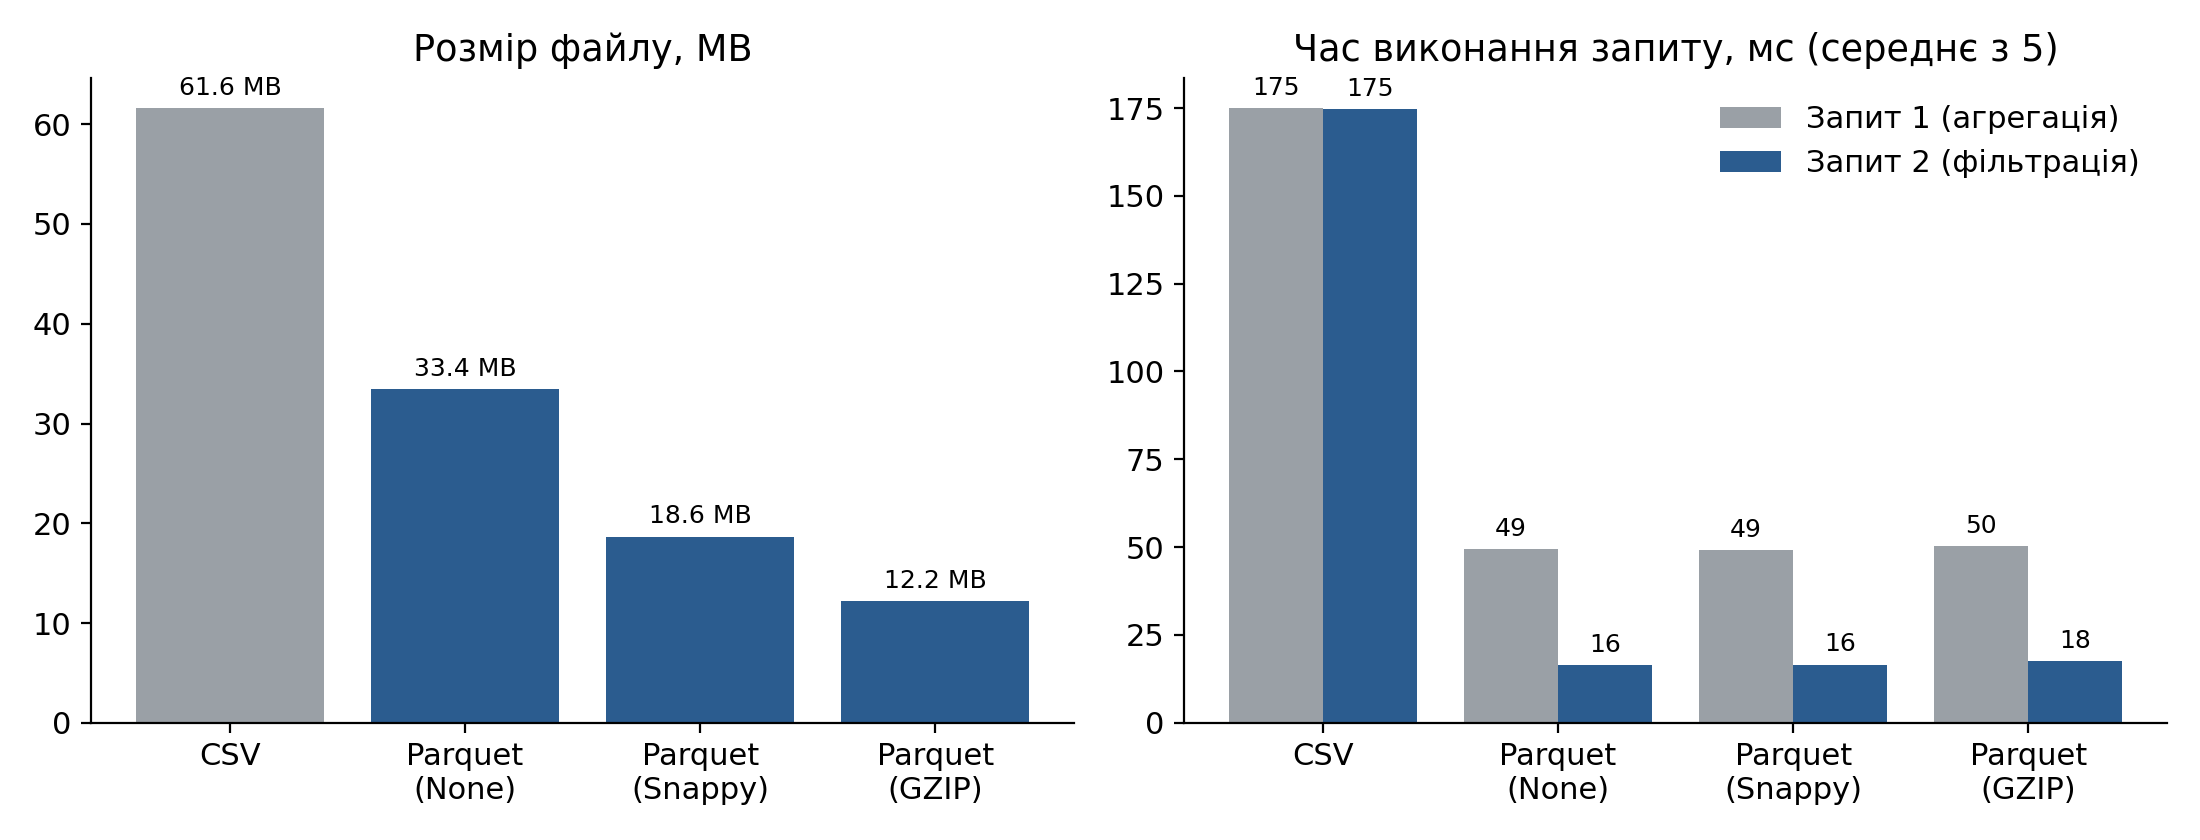
\includegraphics[width=\textwidth]{lab1_results.png}
\caption{Розміри файлів та час виконання запитів для різних форматів}
\label{fig:lab1}
\end{figure}
\end{enumerate}

\rsec{Висновки:} У ході виконання лабораторної роботи №1 набір з 1\,000\,000 транзакцій було перетворено з CSV у Parquet з трьома варіантами стиснення. Parquet без стиснення на 45.7\% менший за CSV, зі Snappy на 69.7\% менший, з GZIP на 80.3\% менший. GZIP дає найменший файл, але запис у ньому найповільніший (0.86~с проти 0.15~с у Snappy). Тому для «гарячих» даних, які часто перезаписуються, доцільний Snappy, а для архівного зберігання GZIP. Аналітичні запити до Parquet виконувалися в 3.5 раза швидше для агрегації та приблизно в 10 разів швидше для фільтрації. Це пояснюється стовпчастою організацією: читаються лише потрібні стовпці, дані не потрібно розбирати з тексту, а фільтр застосовується під час читання. Вибір кодека майже не вплинув на швидкість запитів: витрати на розпакування малі порівняно з виграшем від меншого обсягу вводу-виводу. Отже, для аналітичних навантажень стовпчастий формат зі стисненням суттєво ефективніший за рядковий CSV і за обсягом зберігання, і за швидкістю.

\end{document}
